%%%%%%%%%%%%%%%%%%%%%%%%%%%%%%%%%%%%%%%%%%%%%%%%%%%%%%%%%%%%%%%%%%%%%%%%%%%%%%%
%                       CARREGA DE LA CLASSE DE DOCUMENT                      %
%                                                                             %
% Les opcions admissibles son:                                                %
%      12pt / 11pt            (cos dels tipus de lletra; no feu servir 10pt)  %
%                                                                             %
% catalan/spanish/english     (llengua principal del treball)                 %
%                                                                             % 
% french/italian/german...    (si necessiteu fer servir alguna altra llengua) %
%                                                                             %
% listoffigures               (El document inclou un Index de figures)        %
% listoftables                (El document inclou un Index de taules)         %
% listofquadres               (El document inclou un Index de quadres)        %
% listofalgorithms            (El document inclou un Index d'algorismes)      %
%                                                                             %
%%%%%%%%%%%%%%%%%%%%%%%%%%%%%%%%%%%%%%%%%%%%%%%%%%%%%%%%%%%%%%%%%%%%%%%%%%%%%%%

\documentclass[11pt,spanish,listoffigures,listoftables]{tfgetsinf}

%%%%%%%%%%%%%%%%%%%%%%%%%%%%%%%%%%%%%%%%%%%%%%%%%%%%%%%%%%%%%%%%%%%%%%%%%%%%%%%
%                     CODIFICACIO DEL FITXER FONT                             %
%                                                                             %
%    windows fa servir normalment 'ansinew'                                   %
%    amb linux es possible que siga 'latin1' o 'latin9'                       %
%    Pero el mes recomanable es fer servir utf8 (unicode 8)                   %
%                                          (si el vostre editor ho permet)    % 
%%%%%%%%%%%%%%%%%%%%%%%%%%%%%%%%%%%%%%%%%%%%%%%%%%%%%%%%%%%%%%%%%%%%%%%%%%%%%%%

\usepackage[utf8]{inputenc} 

%%%%%%%%%%%%%%%%%%%%%%%%%%%%%%%%%%%%%%%%%%%%%%%%%%%%%%%%%%%%%%%%%%%%%%%%%%%%%%%
%                        ALTRES PAQUETS I DEFINICIONS                         %
%                                                                        %
% Carregueu aci els paquets que necessiteu i declareu les comandes i entorns  %
%                                          (aquesta seccio pot ser buida)     %
%%%%%%%%%%%%%%%%%%%%%%%%%%%%%%%%%%%%%%%%%%%%%%%%%%%%%%%%%%%%%%%%%%%%%%%%%%%%%%%

\usepackage{graphicx}
\graphicspath{{./figures/}}


%%%%%%%%%%%%%%%%%%%%%%%%%%%%%%%%%%%%%%%%%%%%%%%%%%%%%%%%%%%%%%%%%%%%%%%%%%%%%%%
%                        DADES DEL TREBALL                                    %
%                                                                             %
% titol, alumne, tutor i curs academic                                        %
%%%%%%%%%%%%%%%%%%%%%%%%%%%%%%%%%%%%%%%%%%%%%%%%%%%%%%%%%%%%%%%%%%%%%%%%%%%%%%%

\title{Estrategias de aprendizaje automático aplicadas a videojuegos}
\author{Adrián Valero Gimeno}
\tutor{Vicent Botti Navarro \\
Javier Palanca }
\curs{2018-2019}

%%%%%%%%%%%%%%%%%%%%%%%%%%%%%%%%%%%%%%%%%%%%%%%%%%%%%%%%%%%%%%%%%%%%%%%%%%%%%%%
%                     PARAULES CLAU/PALABRAS CLAVE/KEY WORDS                  %
%                                                                             %
% Independentment de la llengua del treball, s'hi han d'incloure              %
% les paraules clau i el resum en els tres idiomes                            %
%%%%%%%%%%%%%%%%%%%%%%%%%%%%%%%%%%%%%%%%%%%%%%%%%%%%%%%%%%%%%%%%%%%%%%%%%%%%%%%

\keywords{?????????????????} % Paraules clau 
         {Inteligencia artificial, aprendizaje, automatico, videojuegos, OpenAI, hiperparámetros}              % Palabras clave
         {?????, ????? ?????, ?????????????}        % Key words

%%%%%%%%%%%%%%%%%%%%%%%%%%%%%%%%%%%%%%%%%%%%%%%%%%%%%%%%%%%%%%%%%%%%%%%%%%%%%%%
%                              INICI DEL DOCUMENT                             %
%%%%%%%%%%%%%%%%%%%%%%%%%%%%%%%%%%%%%%%%%%%%%%%%%%%%%%%%%%%%%%%%%%%%%%%%%%%%%%%

\begin{document}

%%%%%%%%%%%%%%%%%%%%%%%%%%%%%%%%%%%%%%%%%%%%%%%%%%%%%%%%%%%%%%%%%%%%%%%%%%%%%%%
%              RESUMS DEL TFG EN VALENCIA, CASTELLA I ANGLES                  %
%%%%%%%%%%%%%%%%%%%%%%%%%%%%%%%%%%%%%%%%%%%%%%%%%%%%%%%%%%%%%%%%%%%%%%%%%%%%%%%

\begin{abstract}


Lorem ipsum dolor sit amet, consectetur adipiscing elit. Maecenas semper facilisis rutrum. Nam ullamcorper orci id nisl euismod facilisis. Pellentesque condimentum orci placerat, pulvinar est ut, scelerisque lacus. Pellentesque magna augue, dignissim a tempor in, tincidunt eget mauris. Nunc at sodales nulla. Maecenas congue id sem sagittis mattis. Sed a vehicula justo. Sed rhoncus rutrum ipsum a dictum. Etiam luctus sodales aliquam. Praesent nisl justo, ullamcorper et luctus ut, facilisis vel nibh. Aliquam imperdiet finibus euismod. Donec id posuere libero, eu imperdiet eros. Sed commodo egestas dolor. Ut bibendum turpis mi, vitae iaculis ligula mattis sed. Aliquam dapibus augue et felis pulvinar condimentum vel id mauris. 
\end{abstract}
\begin{abstract}[spanish]


Lorem ipsum dolor sit amet, consectetur adipiscing elit. Maecenas semper facilisis rutrum. Nam ullamcorper orci id nisl euismod facilisis. Pellentesque condimentum orci placerat, pulvinar est ut, scelerisque lacus. Pellentesque magna augue, dignissim a tempor in, tincidunt eget mauris. Nunc at sodales nulla. Maecenas congue id sem sagittis mattis. Sed a vehicula justo. Sed rhoncus rutrum ipsum a dictum. Etiam luctus sodales aliquam. Praesent nisl justo, ullamcorper et luctus ut, facilisis vel nibh. Aliquam imperdiet finibus euismod. Donec id posuere libero, eu imperdiet eros. Sed commodo egestas dolor. Ut bibendum turpis mi, vitae iaculis ligula mattis sed. Aliquam dapibus augue et felis pulvinar condimentum vel id mauris. 
\end{abstract}
\begin{abstract}[english]


Lorem ipsum dolor sit amet, consectetur adipiscing elit. Maecenas semper facilisis rutrum. Nam ullamcorper orci id nisl euismod facilisis. Pellentesque condimentum orci placerat, pulvinar est ut, scelerisque lacus. Pellentesque magna augue, dignissim a tempor in, tincidunt eget mauris. Nunc at sodales nulla. Maecenas congue id sem sagittis mattis. Sed a vehicula justo. Sed rhoncus rutrum ipsum a dictum. Etiam luctus sodales aliquam. Praesent nisl justo, ullamcorper et luctus ut, facilisis vel nibh. Aliquam imperdiet finibus euismod. Donec id posuere libero, eu imperdiet eros. Sed commodo egestas dolor. Ut bibendum turpis mi, vitae iaculis ligula mattis sed. Aliquam dapibus augue et felis pulvinar condimentum vel id mauris. 

\end{abstract}

%%%%%%%%%%%%%%%%%%%%%%%%%%%%%%%%%%%%%%%%%%%%%%%%%%%%%%%%%%%%%%%%%%%%%%%%%%%%%%%
%                              CONTINGUT DEL TREBALL                          %
%%%%%%%%%%%%%%%%%%%%%%%%%%%%%%%%%%%%%%%%%%%%%%%%%%%%%%%%%%%%%%%%%%%%%%%%%%%%%%%

\mainmatter

%%%%%%%%%%%%%%%%%%%%%%%%%%%%%%%%%%%%%%%%%%%%%%%%%%%%%%%%%%%%%%%%%%%%%%%%%%%%%%%
%                                  INTRODUCCIO                                %
%%%%%%%%%%%%%%%%%%%%%%%%%%%%%%%%%%%%%%%%%%%%%%%%%%%%%%%%%%%%%%%%%%%%%%%%%%%%%%%

\chapter{Introducción}

El aprendizaje automático o “Machine Learning” ha sido durante los últimos años el foco de muchísima investigación, debido a su gran potencial en la aplicación a problemas del mundo moderno. En los últimos años, proyectos como AlphaGo o la supercomputadora de google Deep Mind han conseguido hacer grandes avances en juegos de gran dificultad, siendo los agentes desarrollados capaces de competir contra las mentes más experimentadas del tradicional juego de mesa Go. 

Hoy en día se están consiguiendo hacer grandes avances en el campo, debido a la investigación en nuevas técnicas como la combinación de redes neuronales tradicionales con otros métodos como el Deep Learning. Por el momento, Google está liderando este nuevo movimiento, con su supercomputadora DeepMind. Esta computadora fue capaz de desarrollar AlphaGo, una inteligencia artificial capaz de ganar a las mentes más experimentadas del juego tradicional chino Go. Éste juego, considerado uno de los más difíciles del mundo, se calcula que tiene sobre $10^{172}$ configuraciones posibles de las piezas sobre el tablero - un número superior al número estimado de átomos existentes en el universo -, haciéndolo extraordinariamente más complejo que juegos como el ajedrez.




\section{Motivaci\'on}



Se ha elegido un trabajo de estas características debido a una motivación personal hacia los campos de la inteligencia artificial, así como una manera de extender el conocimiento en ciertos ámbitos del mundo de la computación los cuales no se encuentran necesariamente presentes en un plan de estudios tradicional en el campo de la Ingeniería Informática. De esta forma se busca además un desarrollo personal y profesional en el campo de la computación, que permita el acceso a un futuro laboral en éste campo.  \par 

Se partía además de una necesidad personal de realizar un trabajo propio y, de cierta manera, novedoso con respecto a lo que podría conllevar la realización de un proyecto de fin de carrera típico. En definitiva, realizar un trabajo unos objetivos y una metodología a seguir bien definidos y, por encima de todo, que contribuyera al desarrollo de las competencias necesarias para la formación en el campo de la investigación y el desarrollo de sistemas de estas características. 

Inicialmente, la idea para realizar el trabajo surgió meses antes de comenzar el trabajo per se, y consistía en la realización de algoritmos especializados para el aprendizaje de Cuphead, un videojuego del año 2017 con características similares a los juegos en 2D de antaño. Después de realizar una investigación exhaustiva de las maneras que tendríamos que enfocar el problema, observamos que dado que no se trata de un juego con un entorno accesible para la realización de nuestro trabajo. Esto es debido a restricciones como el código propietario, el alto nivel de dificultad de la mayoría de sus niveles y el hecho de que requiere unas grandes cantidades de tiempo y recursos de entrenamiento, al no ser posible de ejecutar fácilmente de manera asíncrona sin un alto coste de recursos computacionales. 

\section{Objetivos}

El propósito de este TFG consistirá en el estudio de las diferentes técnicas existentes de aprendizaje automático aplicadas a sencillos videojuegos en 2D, los cuales tendrán un número limitado de acciones a realizar. Se pretende además, realizar implementaciones propias de las diferentes técnicas descritas durante el resto del documento. \par 

Otro de los objetivos consistirá en el estudio y realización de pruebas sobre distintos entornos predefinidos de juegos arcade, haciendo uso de librerías que permiten el acceso a dicho tipo de juegos como la herramienta OpenAI desarrollada por Google, o las distintas librerías de Python relacionadas con la creación de entornos de redes neuronales y, más concretamente, la manipulación de hiperparámetros para encontrar los mejores resultados para cada uno de los entornos estudiados. \par 

% Otra idea puede ser el Doom
Por último, resultaría interesante aplicar estas nuevas técnicas estudiadas en la resolución de algún videojuego de mayor complejidad. Se plantea, por lo tanto, un estudio de los algoritmos más destacables estudiados en algún juego complejo como puede ser Montezuma's Revenge, un juego de la atari 2600 estrenado en el año 1983.


\section{Metodología}

Para la realización de este trabajo se pretende llevar a cabo una investigación en el campo de la inteligencia artificial, concretamente en el desarrollo de algoritmos de aprendizaje aplicados a entornos estocásticos. Para ello, se investigarán técnicas como el aprendizaje por refuerzo o Q-Learning, algoritmos evolutivos, o el uso de redes neuronales. Adicionalmente, se ha seguido un curso externo enfocado a la teoría de inteligencia artificial aplicada a distintos videojuegos, en los cuales se introducen los conceptos principales en los cuales se basa todo el campo del aprendizaje por refuerzo, desde la ecuación de Bellman hasta el diseño de redes neuronales convolucionales como método para acceder a la información de nuestros entornos. \par

Para complementar nuestra base de conocimientos, nos basaremos en artículos de investigación publicados por entidades como Google DeepMind, o el Massachussets Institute of Technology, en busca de ideas y nuevas técnicas para su posterior aplicación en nuestro trabajo.


\section{Estructura de la memoria}

????? ????????????? ????????????? ????????????? ????????????? ????????????? 

%\section{Notes bibliografiques} %%%%% Opcional

%????? ????????????? ????????????? ????????????? ????????????? ?????????????

%%%%%%%%%%%%%%%%%%%%%%%%%%%%%%%%%%%%%%%%%%%%%%%%%%%%%%%%%%%%%%%%%%%%%%%%%%%%%%%
%                         CAPITOLS (tants com calga)                          %
%%%%%%%%%%%%%%%%%%%%%%%%%%%%%%%%%%%%%%%%%%%%%%%%%%%%%%%%%%%%%%%%%%%%%%%%%%%%%%%


\chapter{Estado del arte. La situación del aprendizaje automático en la actualidad}

\section{Introducción al Q-Learning}

%% Se puede ahondar MUCHO MÁS en este campo de la neurociencia
El aprendizaje por refuerzo o \textit{Q-Learning} es un principio altamente utilizado en la actualidad en la investigación del campo de la Inteligencia Artificial. Este enfoque se inspira en el campo de la psicología de comportamiento y pone el énfasis en cómo un agente independiente será capaz de tomar las acciones pertinentes basándose en un sistema de recompensas a partir de las acciones que toma. \par 

Debido a la capacidad creciente de los ordenadores de realizar computaciones cada vez más complejas en cantidades de tiempo exponencialmente menores, así como la facilidad de acceso a la información que han permitido factores como internet o, en igual medida, el abaratamiento creciente de sistemas de almacenamiento con respecto a décadas anteriores, se plantea el problema de que disponemos de un acceso a la información demasiado grande para ser tratado por métodos tradicionales. 

En los últimos años, se ha podido observar un crecimiento notable en el uso de sistemas de inteligencia artificial en empresas de internet hasta el punto en el que se han convertido en un requisito casi indispensable para ser capaz de ofrecer un servicio específico; por ejemplo, los sistemas de recomendación en servicios de plataformas de Streaming o la publicidad personalizada que muchas páginas de compras por internet ofrecen basándose en las compras o búsquedas realizadas anteriormente. Estos sistemas se basan en el entrenamiento de redes neuronales que permiten crear una relación entre las selecciones anteriores y productos afines.

\subsection{Los elementos del Aprendizaje por refuerzo}

Como se ha mencionado anteriormente, el aprendizaje por refuerzo se basa en ideas de la neurociencia y la psicología, específicamente del campo de la psicología del comportamiento. 

%Hablar de Policy, Reward Function, Value function, modelo del entorno (a partir de la pagina 16 \cite{neural_rl})

Se pueden identificar cuatro subelementos esenciales en un sistema de aprendizaje por refuerzo. Estos elementos son: \textit{política, función de recompensa}, un \textit{modelo de entorno} bien definido y lo que llamaremos \textit{función de valía}.

Una \textit{política} definirá el comportamiento de el agente en cuestión en un momento determinado. Consistirá pues, en un mapeado de los estados que se han percibido hasta el momento en relación a las acciones tomadas en el pasado. En psicología, se correspondería a lo que es llamado una serie de reglas de estímulo respuesta. Esta política podrá venir dada de diferentes maneras, desde una simple tabla de resultados a una serie de computaciones llevadas a cabo en una red neuronal.

La \textit{función de recompensa} a su vez definirá el objetivo del problema. Consistirá en una colección de relaciones estado-acción a las que se les asignará un valor numérico individual, dependiendo de si la acción tomada en un estado dado es favorable o no para la consecución del objetivo. El objetivo del agente será siempre intentar maximizar la recompensa total obtenida en un episodio\footnote{Al hablar de episodio, nos referimos a una determinada secuencia de estados dentro de un entorno hasta dar con un estado final.}.

Mientras que la función de recompensa nos indicará la recompensa inmediata que un agente recibirá al realizar una determinada acción, la \textit{función de valía} o Q-Value nos especificará el valor esperado de recompensa que se conseguirá al seguir una serie de acciones que, a priori, podrían no parecer las óptimas, pero pueden ser ventajosas a medio o largo plazo. Éste valor puede resultar muy complicado de calcular, y requiere una capacidad de cómputo enorme que aumenta exponencialmente en entornos con un gran número de dimensiones. Esto se traduce en una dificultad real - y que todavía no se ha sido capaz de solventar - de los agentes de planear acciones a medio o largo plazo. 

En último lugar, el \textit{modelo del entorno}


%Hablar tambien de loss function (IMPORTANTE)

\subsection{Cadenas de Markov}

Este enfoque se basa en la consideración del problema a resolver como un proceso de decisión de Markov con recompensa (MRP), es decir, una tupla (S, P, R, $\gamma$) donde $S_{n}$ denota el estado posible \textbf{S}  en el que un agente se puede encontrar, $P_{n}$ una función de transición \textbf{P} y $R_{n}$ es la recompensa que un agente conseguirá al realizar una determinada acción. Por último, $\gamma$ denotará el factor de descuento donde $\gamma \in [0,1]$. Éste parámetro indica al agente cuanto peso debe darle a las recompensas que recibe para aplicar estos conocimientos en momentos posteriores del aprendizaje. Se ha observado en diferentes investigaciones que introducir un factor de descuento de 1 no garantizará necesariamente la convergencia, por lo que resulta recomendable dotar al agente de cierta autonomía para la exploración, que podría resultar en el descubrimiento de acciones más ventajosas a la hora de resolver un problema determinado. De esta manera, la noción en la que el agente percibirá la señal de recompensa \textbf{$R(s,a)$} vendrá dada por:
\[R(s,a) = R_{t+1} + \gamma^{2}R_{t+2} + ... + \gamma^{n-t}R_{n} = \displaystyle\sum_{k=0}^{n} \gamma^{k} R_{t+k+1} \]

El objetivo de nuestro agente será en todo momento conseguir maximizar la recompensa total obtenida en un episodio, basándose en el principio de la ecuación anterior para determinar los posibles caminos a seguir. De esta manera, la función de recompensa final podrá ser expresada como:  \[V(s) = max_{a}[R(s,a) + \gamma \sum{s'}P(s,a,s') V(s')]\]
%\[V(s) = max_{a}(R(s,a) + \gamma V(s'))\]

%// aqui ira algo más

%Uno de los principales problemas de éste tipo de sistemas consiste en la imposibilidad de los agentes de extrapolar el conocimiento recibido a 

\subsection{Redes neuronales}

El concepto de red neuronal nace de la idea de conseguir un comportamiento autónomo similar al de un ser humano. De esta manera, las redes neuronales intentan replicar el razonamiento humano creando una relación entre lo que el agente observa y las acciones que ha de realizar. Dependiendo del problema a abarcar, estas redes se pueden ver reformuladas para ajustarse a una serie de requerimientos especiales. Por ejemplo, las redes neuronales convolucionales hacen uso de una serie de capas previas que extraen características de las imágenes para ser posteriormente introducidas en una estructura de red neuronal clásica y realizar así la tarea de clasificación.

Una red neuronal se compone esencialmente de tres componentes interconectados: Una capa de entrada, una o varias capas ocultas, y una capa de salida.

\begin{figure}[h]
	\centering
	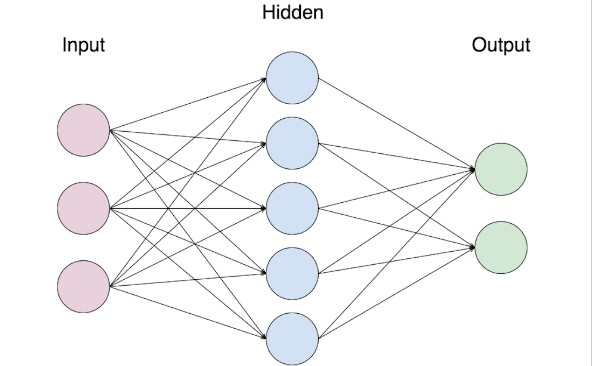
\includegraphics[scale=0.4]{fig_neuralnetwork}
	\caption{Ejemplo de una red neuronal con una capa oculta de 5 nodos (neuronas).}
	
\end{figure}

Con respecto a las neuronas, su valor se extraerá de realizar una suma de las señales que recibe, para ser pasadas posteriormente por una función de activación. Normalmente, a este sumatorio se le agrega un valor llamado prejuicio (\textit{bias}). Se ha demostrado que esta adición puede reducir el tiempo necesario de entrenamiento de una red neuronal.

Este sistema toma una serie señales introducidas a través de la capa de entrada, normalizadas a unos pesos independientes entre si con valores entre 0 y 1, que a su vez emitirán estas señales a cada una de las neuronas de la primera capa oculta. Aquí, las señales tendrán que pasar por una \textbf{función de activación} que determinará si esa neurona se activa o no, para después pasar la respectiva señal a la siguiente capa. Finalmente, se obtendrá un valor de salida de las neuronas de la última capa correspondiente a 0 o 1, dependiendo de la clasificación que la red haya determinado. Este concepto se conoce como \textit{forward-propagation}.

Dado que nuestro entorno se trata de un entrono de \textbf{aprendizaje supervisado}, se puede determinar el valor correcto que las capas exteriores deben tomar. El concepto del \textit{backpropagation} utiliza esta ventaja que nos ofrecen los entornos deterministas para realizar así una correción de cómo el sistema maneja las señales de entrada. Así, la red neuronal es capaz de ajustar sus funciones de activación para poder realizar una mejor clasificación en pruebas posteriores.

\subsection{El concepto de Q-Learning}



\subsection{Redes convolucionales (CNNs)}

Las redes neuronales clásicas no están preparadas para soportar inputs de imágenes, ya que las señales de entrada necesitan tener ya unos valores numéricos normalizados. Por ello es necesario que las imágenes pasen por un tratamiento previo a su introducción en una red neuronal clásica. Este tipo de sistemas se llaman redes neuronales convolucionales.

El preprocesamiento de imágenes llevado a cabo en este tipo de imágenes viene ilustrado en la siguiente figura:

\begin{figure}[h]
	\centering
	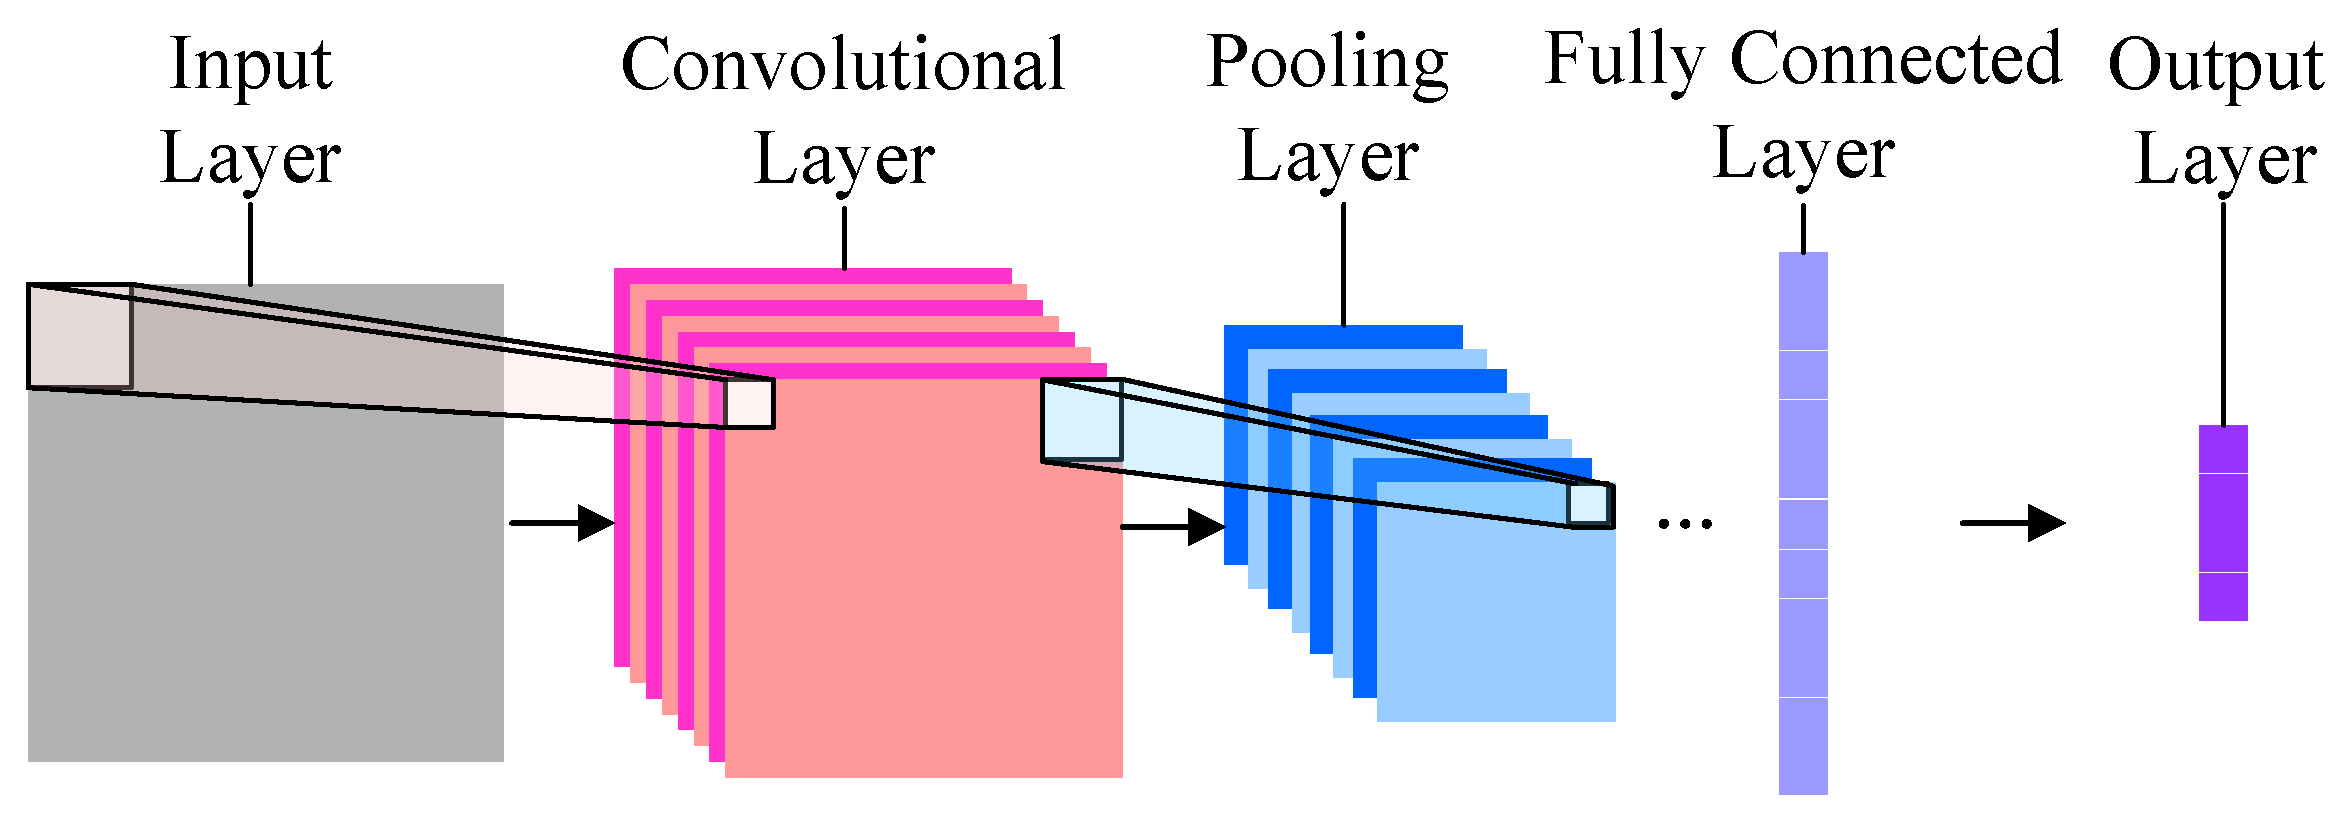
\includegraphics[]{CNNStructure}
	\caption{Ejemplo de red convolucional}
	
\end{figure}

Como se puede observar, la red se puede dividir en diferentes capas:

\begin{description}
	\item[Capa convolucional o detector de características.] Se utiliza para filtrar la imagen de entrada de manera que el resultado sea una matriz de menor orden conteniendo las características de la imagen que sean útiles para la clasificación. Normalmente se aplican diferentes filtros en búsqueda de diversas características, que luego se agrupan y se pasan a la siguiente capa.
	\item [Capa de agrupamiento.] Reduce de nuevo el tamaño de la matriz de características, extrayendo de ella la información más remarcable de cada grupo de píxeles. De esta manera, se puede reducir el tamaño de la imagen hasta en un 75\%.
	\item[Capa de aplanamiento.] Adicionalmente, se utiliza una capa extra que toma los mapas de características resultantes de la capa de agrupamiento y crea con ellos una matriz de tamaño n x 1, que a su vez será la capa de entrada de la red neuronal.
\end{description}

\subsection{El problema de la memoria. El \textit{experience replay}}

Normalmente, para una correcto aprendizaje en entornos estocásticos\footnote{Un entorno estocástico es aquel con un número finito de estados definidos.}, no basta con la implementación de una red neuronal. En su definición más simple, los algoritmos de aprendizaje descartan la información respectiva a experiencias anteriores inmediatamente después de decidir la acción a tomar.

Resulta útil un mecanismo que sea capaz de almacenar y usar de nuevo las experiencias pasadas del agente, ya que soluciona distintos problemas que pueden surgir si no se sigue este enfoque. Por ejemplo, es interesante el tener constancia de estados poco comunes que requieran unas acciones específicas para conseguir un resultado favorable en posteriores iteraciones. Este mecanismo es el denominado \textit{experience replay}.

El resultado de realizar una implementación de estas características constituye en una menor necesidad de los agentes de experiencias para converger, a cambio de poder de cómputo y almacenamiento de datos - recursos accesibles con un menor coste temporal.

Adicionalmente, \cite{exp_replay_prior} argumenta que priorizar las experiencias que el agente accede en memoria puede tener un efecto positivo en la rápida convergencia del aprendizaje, partiendo de la idea de que existirán experiencias de las que el agente podrá aprender de manera más efectiva que otras, o bien existir algunas que puedan no ser útiles para un estado determinado y que más tarde pasen a ser vitales para la correcta ejecución de cierta secuencia de acciones. El principal problema de esta ordenación por prioridad será entonces determinar el criterio por el cual se mide la importancia de cada transición de estados. Idealmente, esto se realizaría tomando como criterio la cantidad de información que el agente puede aprender de la transición desde el estado actual. Sin embargo, este no es un factor que podamos calcular. En su lugar, una aproximación adecuada podría ser tomar el error TD de una transición $\delta$, lo cual nos daría una noción de cómo de 'sorprendente' o innovadora determinada acción resultará.

Esta solución no viene sin problemas, ya que este algoritmo de priorización acabará centrándose en un pequeño grupo de experiencias que se repetirán de manera frecuente. Además el error se reducirá lentamente con el paso de cada iteración, lo cual podría desembocar a su vez en problemas de sobreajuste\footnote{El sobreajuste o \textit{overfitting} en inglés, es el efecto de sobreentrenar un algoritmo de aprendizaje para encontrar soluciones que ya se conocen.}.

\cite{exp_replay_prior} concluye después de realizar experimentaciones en el entorno de Atari 2600, que una correcta implementación del \textit{experience replay} basado en prioridades podría aumentar el aprendizaje conseguido por un factor de 2.



\section{Historia de la evolución tecnológica}

\section{Aplicación en videojuegos}



\section{Algoritmos existentes en la actualidad}



\chapter{??? ???? ??????}

????? ????????????? ????????????? ????????????? ????????????? ????????????? 

\section{?? ???? ???? ? ?? ??}

????? ????????????? ????????????? ????????????? ????????????? ?????????????

%%%%%%%%%%%%%%%%%%%%%%%%%%%%%%%%%%%%%%%%%%%%%%%%%%%%%%%%%%%%%%%%%%%%%%%%%%%%%%%
%                                 CONCLUSIONS                                 %
%%%%%%%%%%%%%%%%%%%%%%%%%%%%%%%%%%%%%%%%%%%%%%%%%%%%%%%%%%%%%%%%%%%%%%%%%%%%%%%

\chapter{Conclusions}

????? ????????????? ????????????? ????????????? ????????????? ????????????? 

%%%%%%%%%%%%%%%%%%%%%%%%%%%%%%%%%%%%%%%%%%%%%%%%%%%%%%%%%%%%%%%%%%%%%%%%%%%%%%%
%                                BIBLIOGRAFIA                                 %
%%%%%%%%%%%%%%%%%%%%%%%%%%%%%%%%%%%%%%%%%%%%%%%%%%%%%%%%%%%%%%%%%%%%%%%%%%%%%%%

\begin{thebibliography}{10}

%%%%%%%%%%%%%%%%%%%%%%%%%%%%%%%%%%%%%%%%%%%%%%%%%%%%%%%%%%%%%%%%%%%%%%%%%%%%%%%
% MODEL D'ARTICLE                                                             %
%%%%%%%%%%%%%%%%%%%%%%%%%%%%%%%%%%%%%%%%%%%%%%%%%%%%%%%%%%%%%%%%%%%%%%%%%%%%%%%
\bibitem{light}
   Jennifer~S. Light.
   \newblock When computers were women.
   \newblock \textit{Technology and Culture}, 40:3:455--483, juliol, 1999.

%%%%%%%%%%%%%%%%%%%%%%%%%%%%%%%%%%%%%%%%%%%%%%%%%%%%%%%%%%%%%%%%%%%%%%%%%%%%%%%
% MODEL DE LLIBRE                                                             %
%%%%%%%%%%%%%%%%%%%%%%%%%%%%%%%%%%%%%%%%%%%%%%%%%%%%%%%%%%%%%%%%%%%%%%%%%%%%%%%
\bibitem{ifrah}
   Georges Ifrah.
   \newblock \textit{Historia universal de las cifras}.
   \newblock Espasa Calpe, S.A., Madrid, sisena edició, 2008.

%%%%%%%%%%%%%%%%%%%%%%%%%%%%%%%%%%%%%%%%%%%%%%%%%%%%%%%%%%%%%%%%%%%%%%%%%%%%%%%
% MODEL D'URL                                                                 %
%%%%%%%%%%%%%%%%%%%%%%%%%%%%%%%%%%%%%%%%%%%%%%%%%%%%%%%%%%%%%%%%%%%%%%%%%%%%%%%
\bibitem{WAR}
   Comunicat de premsa del Departament de la Guerra, 
   emés el 16 de febrer de 1946. 
   \newblock Consultat a 
   \url{http://americanhistory.si.edu/comphist/pr1.pdf}.
   
\bibitem{methods_RL}
	Volodymyr Mnih, Adrià Puigdomènech Badia, Mehdi Mirza, Alex Graves, Tim Harley, Timothy P. Lillicrap, David Silver, Koray Kavukcuoglu.
	\newblock Asynchronous Methods for Deep Reinforcement Learning,
	febrero de 2016.
	\newblock \textit {Google DeepMind, Montreal Institute for Learning Algorithms (MILA), University of Montreal}
	
\bibitem{Tokic}
	Michel Tokic
	\newblock Adaptive $\varepsilon$-greedy Exploration in Reinforcement Learning Based on Value Differences.
	\newblock \textit {Institute of Applied Research, University of Applied Sciences Ravensburg-Weingarten, 88241 Weingarten, Germany}
	
\bibitem{Wu}
	Jianxin Wu
	\newblock Introduction to Convolutional Neural Networks,
	mayo de 2017.
	\newblock \textit {LAMDA Group \newblock National Key Lab for Novel Software Technology. Nanjing University, China}
	
\bibitem{exp_replay_prior}
	Tom Schaul, John Quan, Ioannis Antonoglou, David Silver
	\newblock Prioritized Experience Replay,
	febrero de 2016.
	\newblock \textit {Google DeepMind}
	
\bibitem{neural_rl}
	 Wolfram Schultz, Peter Dayan, P. Read Montague
	 \newblock A Neural Substrate of Prediction and Reward
	 Science 275, 1593-1599 (1997)
	 
\bibitem{dqn}
	Varios autores
	\newblock Human-level control through deep reinforcement learning
	\newblock \textit{Nature}, vol 518, 26 de febrero de 2015

\end{thebibliography}
\cleardoublepage

%%%%%%%%%%%%%%%%%%%%%%%%%%%%%%%%%%%%%%%%%%%%%%%%%%%%%%%%%%%%%%%%%%%%%%%%%%%%%%%
%                           APÈNDIXS  (Si n'hi ha!)                           %
%%%%%%%%%%%%%%%%%%%%%%%%%%%%%%%%%%%%%%%%%%%%%%%%%%%%%%%%%%%%%%%%%%%%%%%%%%%%%%%

\APPENDIX

%%%%%%%%%%%%%%%%%%%%%%%%%%%%%%%%%%%%%%%%%%%%%%%%%%%%%%%%%%%%%%%%%%%%%%%%%%%%%%%
%                         LA CONFIGURACIO DEL SISTEMA                         %
%%%%%%%%%%%%%%%%%%%%%%%%%%%%%%%%%%%%%%%%%%%%%%%%%%%%%%%%%%%%%%%%%%%%%%%%%%%%%%%

\chapter{Configuració del sistema}

????? ????????????? ????????????? ????????????? ????????????? ?????????????

\section{Fase d'inicialització}

????? ????????????? ????????????? ????????????? ????????????? ?????????????

\section{Identificació de dispositius}

????? ????????????? ????????????? ????????????? ????????????? ?????????????

%%%%%%%%%%%%%%%%%%%%%%%%%%%%%%%%%%%%%%%%%%%%%%%%%%%%%%%%%%%%%%%%%%%%%%%%%%%%%%%
%                               ALTRES  APÈNDIXS                              %
%%%%%%%%%%%%%%%%%%%%%%%%%%%%%%%%%%%%%%%%%%%%%%%%%%%%%%%%%%%%%%%%%%%%%%%%%%%%%%%


\chapter{??? ???????????? ????}

????? ????????????? ????????????? ????????????? ????????????? ????????????? 



%%%%%%%%%%%%%%%%%%%%%%%%%%%%%%%%%%%%%%%%%%%%%%%%%%%%%%%%%%%%%%%%%%%%%%%%%%%%%%%
%                              FI DEL DOCUMENT                                %
%%%%%%%%%%%%%%%%%%%%%%%%%%%%%%%%%%%%%%%%%%%%%%%%%%%%%%%%%%%%%%%%%%%%%%%%%%%%%%%

\end{document}
